% !TeX document-id = {0be8c18c-9430-4e9a-bdd9-12beadebfebc}
% !TeX TXS-program:bibliography = txs:///biber
\documentclass[11pt]{beamer}
\uselanguage{portuguese}
\languagepath{portuguese}
\deftranslation[to=portuguese]{Theorem}{Teorema}
\deftranslation[to=portuguese]{theorem}{teorema}
\deftranslation[to=portuguese]{Example}{Exemplo}
\deftranslation[to=portuguese]{example}{exemplo}
\deftranslation[to=portuguese]{Lemma}{Lema}
\deftranslation[to=portuguese]{lemma}{Lema}
\deftranslation[to=portuguese]{Corollary}{Corolário}
\deftranslation[to=portuguese]{corollary}{corolário}
%\deftranslation[to=portuguese]{and}{e}

\usepackage[brazilian]{babel}
\usepackage[utf8]{inputenc}
\usepackage[T1]{fontenc}
\usepackage{lmodern}
\usepackage{amsmath}
\usepackage{amssymb}
\usepackage{mathtools}
\usepackage{color}
\usepackage{pgfplots}
\usepackage{tikz}

%\usepackage{appendixnumberbeamer}

\newenvironment{transitionframe}{
	\setbeamercolor{background canvas}{bg=yellow}
	\begin{frame}}{
	\end{frame}
}
\usetheme{default}
\usefonttheme{structuresmallcapsserif}

%% I use a beige off white for my background
\definecolor{MyBackground}{RGB}{255,253,218}
\useinnertheme[shadow]{rounded}
\setbeamercolor{block title}{bg=MyBackground}
\setbeamercolor{block body}{bg=MyBackground}
\setbeamercolor{example title}{bg=MyBackground}
\setbeamercolor{example body}{bg=MyBackground}


\newcommand{\blue}[1]{\textcolor{blue}{#1}}
\newcommand{\red}[1]{\textcolor{red}{#1}}
\newcommand{\purple}[1]{\textcolor{purple}{#1}}
\newcommand{\gray}[1]{\textcolor{gray}{#1}}
\setbeamertemplate{navigation symbols}{}
%\setbeamertemplate{page number in head/foot}[appendixframenumber]

%\usepackage{graphics}
\usepackage{graphicx}

\definecolor{blue_emph}{RGB}{0,114,178}
\definecolor{red}{RGB}{213,94,0}
\definecolor{yellow}{RGB}{240,228,66}
\definecolor{green}{RGB}{0,158,115}
\definecolor{purple}{RGB}{204,121,167}
\definecolor{orange}{RGB}{230,159,0}
\definecolor{lightblue}{RGB}{86,180,233}

%\setbeamercolor{frametitle}{fg=blue}
%\setbeamercolor{title}{fg=blue}
\setbeamertemplate{footline}[frame number]
\setbeamertemplate{navigation symbols}{} 
\setbeamertemplate{itemize items}{-}
%\setbeamercolor{itemize item}{fg=blue}
%\setbeamercolor{itemize subitem}{fg=blue}
\setbeamertemplate{enumerate items}[default]
%\setbeamercolor{enumerate subitem}{fg=blue}
\setbeamercolor{button}{bg=MyBackground,fg=blue}
\usefonttheme{structuresmallcapsserif}

%\setbeamercolor{section in toc}{fg=blue}
%\setbeamercolor{subsection in toc}{fg=red}
\setbeamersize{text margin left=1em,text margin right=1em} 


\usepackage{appendixnumberbeamer}

\usepackage[
backend=biber,
style=authoryear,
natbib=true,
uniquename=false,
]{biblatex}
\addbibresource{../bibliography.bib}

\newenvironment{wideitemize}{\itemize\addtolength{\itemsep}{10pt}}{\enditemize}
\newenvironment{wideenumerate}{\enumerate\addtolength{\itemsep}{10pt}}{\endenumerate}
\newenvironment{halfwideitemize}{\itemize\addtolength{\itemsep}{0.5em}}{\enditemize}
\newenvironment{halfwideenumerate}{\enumerate\addtolength{\itemsep}{0.5em}}{\endenumerate}


\author{Luis A. F. Alvarez}
\title{Introdução à Econometria Semiparamétrica}
\subtitle{Aula 3 - Estimação Semiparamétrica}
%\logo{}
%\institute{}
\date{\today}
%\subject{}
%\setbeamercovered{transparent}

\begin{document}

	\begin{frame}[plain]
	\maketitle
	\end{frame}

	
	\begin{frame}{Exemplo}
		\begin{itemize}
			\item Considere uma população de interesse em que definimos um tratamento individual binário, denotado por uma variável aleatória, $D \in \{0,1\}$ e um resultado de interesse $Y$.
			\begin{itemize}
				\item Os resultados potenciais, que descrevem o que acontece com um indivíduo caso ele seja alocado ao tratamento ou não, são dados por $(Y(0),Y(1))$, de modo que o resultado observado é dado por $Y = DY(1)+(1-D)Y(0)$ e o efeito da política é $Y(1)-Y(0)$ .
			\end{itemize}
			\item Sejam $X$ um vetor de características observáveis, tais que seja razoável supor que:
			
			$$Y(0)\perp D | X$$
		\end{itemize}
	\end{frame}
	\begin{frame}{Estimação do ATT}
		\begin{itemize}
			\item Sob a hipótese de identificação anterior, se supomos que 	$\mathbb{P}[D=1]> 0$ e a seguinte hipótese de suporte comum (\textit{overlap}):
			
			$$\exists \epsilon > 0, \quad \mathbb{P}[\mathbb{P}[D=0|X]\geq \epsilon] = 1 $$
		
			\item Então é possível identificar o efeito médio do tratamento nos tratados (ATT), 
			{\small$$ \mathbb{E}[Y(1)-Y(0)|D=1] = \frac{\mathbb{E}[DY]}{\mathbb{E}[D]} - \frac{1}{\mathbb{E}[D]}\mathbb{E}\left[\frac{\mathbb{P}[D=1|X=1]}{1-\mathbb{P}[D=1|X=1]}(1-D)Y\right]$$}
			\item O problema é que a hipótese de suporte comum pode ser irrazoável em alguns contextos.
		\end{itemize}
	\end{frame}
	
	\begin{frame}{Combinações convexas de ATTs condicionais}
		\begin{itemize}
			\item Considere, como alternativa, o estimando $\beta^*$ que resolve
			
			$$(\beta^*,g) = \operatorname{argmin}_{{b\in \mathbb{R}, h \in \mathcal{H}}} \mathbb{E}[(Y-bD - h(X))^2]\, ,$$
			onde $\mathcal{H}$ é um sub-espaço fechado de $L_2(\mathbb{P}_X)$.
			\item Nesse caso, é possível mostrar que, {\color{blue}se $\mathbb{P}[D=1|X]\in \mathcal{H}$ ou $\mathbb{E}[Y(0)|X] \in \mathcal{H}$}, então:
			
			$$\beta^* = \frac{\mathbb{E}[\mathbb{E}[Y(1)-Y(0)|X,D=1]\mathbb{P}[D=1|X](1-m(X)) ]}{\mathbb{E}[\mathbb{P}[D=1|X](1-m(X)) ]}$$
			onde $m(X) = \operatorname{argmin}_{h \in \mathcal{H}} \mathbb{E}[(D-h(X))^2]$.
			\item Resultado é extensão direta de \citet{Angrist1998}. \hyperlink{proof_angrist}{\beamergotobutton{Detalhes}}
			\label{main}
			\item Se  $m(X) \in [0,1]$ com probabilidade 1, estimando é uma combinação convexa de ATTs condicionais, dando mais peso para pontos do suporte com melhor sobreposição.
			\begin{itemize}
				\item Combinação convexa mais fácil de se estimar eficientemente \citep{contaminationbias}, sob algumas hipóteses.
			\end{itemize}
		\end{itemize}
	\end{frame}
	
	\begin{frame}{Estimando $\beta^*$}
		\begin{itemize}
			\item Com base no resultado anterior e uma amostra aleatória da população, poderíamos tentar estimar $\beta^*$ resolvendo o análogo amostral do problema.
			\begin{itemize}
				\item Para implementar classes ``complexas'' $\mathcal{H}$, podemos alternar o estimador de MQO dos resíduos $(Y_i-\tilde{g}(X_i))$ em $D_i$ e o estimador que projeta $Y_i - \tilde{\beta} D_i$ em $\mathcal{H}$ até convergência.
			\end{itemize} 
			\item Note, entretanto, que para a representação anterior valer, devemos escolher uma classe suficiente expressiva para representar ou $\mathbb{E}[Y(0)|X]$ ou $\mathbb{P}[D=1|X]$.
			\begin{itemize}
				\item Especificamente, se $X$ contém variável contínua com suporte na reta que é relevante para a seleção, então classe linear não será capaz de satisfazer $m(X) \in [0,1]$ com probabilidade 1, e não teremos combinação convexa de ATTs (pesos negativos).
				\item Além disso, se há muitos possíveis controles, mas somente um subconjunto é relevante para explicar a seleção ao tratamento, deveríamos utilizar métodos de alta dimensão válidos sob esparsidade. 
			\end{itemize}
			\item Estimador resultante é dado por:
			\vspace{-0.5em}
			$$\hat{\beta} = \frac{ \frac{1}{n} \sum_{i=1}^nD_i (Y_i - \hat{g}(X_i))}{\frac{1}{n}\sum_{i=1}^n D_i^2}\, .$$
		\end{itemize}
	\end{frame}
	
	\begin{frame}{Aproximação assintótica do estimador}
		\begin{equation*}
			\footnotesize 
			\begin{aligned}
						\sqrt{n}\left(\hat{\beta}-\beta^*\right)=\\ \underbrace{\left(\frac{1}{n} \sum_{i \in I} D_{i}^{2}\right)^{-1} \frac{1}{\sqrt{n}} \sum_{i \in I} D_{i} U_{i}}_{=:a}+\underbrace{\left(\frac{1}{n} \sum_{i \in I} D_{i}^{2}\right)^{-1} \frac{1}{\sqrt{n}} \sum_{i \in I} D_{i}\left(g\left(X_{i}\right)-\hat{g}\left(X_{i}\right)\right)}_{=:b}
			\end{aligned}
		\end{equation*}
						onde $U_i = Y_i - \beta^* D_i - g(X_i)$.

		\begin{itemize}
			\item Termo $a$ é bem comportado em amostras grandes $a\overset{d}{\to} N(0,\sigma^2)$.
			\item No entanto, termo $b$ é dado por:
			\(b=\left(E\left[D_{i}^{2}\right]\right)^{-1} \frac{1}{\sqrt{n}} \sum_{i \in I} m\left(X_{i}\right)\left(g\left(X_{i}\right)-\hat{g}\left(X_{i}\right)\right)+o_{P}(1)\)
			\item Esse termo não é bem comportado para estimadores não paramétricos, especialmente modernos.
			\begin{itemize}
				\item Comparar EQM do MQO com outras alternativas que operam no trade-off viés variância.
				\begin{itemize}
				\item No MQO, $\sqrt{n}(\hat{\delta}'x - \delta_0'x) \overset{d}{\to}N(0, x'\Sigma^2_{\hat{\delta}}x)$, de modo que esperamos que, em amostras grandes, $\infty>\mathbb{V}[b] > 0$, mas $\mathbb{E}[b]\approx 0$.
				\item Para estimadores não paramétricos modernos que operam no tradeoff vié-variância $\mathbb{E}[b] = \frac{1}{n^{-1/2 + \psi}}$, para $\psi < 1/2$ (ver exemplo do Lasso). 
				\item Distribuição arbitrariamente não centrada em $\beta^*$ em amostras grandes.
				 \end{itemize}
			\end{itemize}
		\end{itemize}
	\end{frame}
	
	\begin{frame}{Exemplo: viés  na distribuição do estimador semiparamétrico ``ingênuo''}
	\centering
	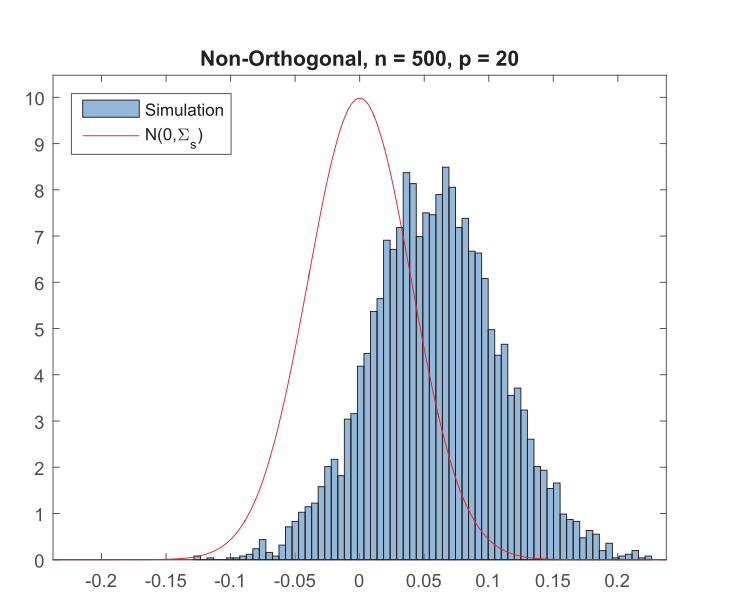
\includegraphics[scale=0.5]{graficos/naive.png}
	\end{frame}
	\begin{frame}{Estimador alternativo}
		\begin{itemize}
			\item É possível mostrar que parâmetro de interesse pode ser identificado como:
			
			$$\beta^*  =  \frac{\mathbb{E}[(Y - g(X))(D-m(X)) ]}{\mathbb{E}[(D-m(X))D]}$$
			\item Considere então:
			
			$$\check{\beta}=\left(\frac{1}{n} \sum_{i \in I} \hat{V}_{i} D_{i}\right)^{-1} \frac{1}{n} \sum_{i \in I} \hat{V}_{i}\left(Y_{i}-\hat{g}\left(X_{i}\right)\right)\,, $$
			onde $\hat{V}_i = D_i - \hat{m}(X_i)$.

			
		\end{itemize}
	\end{frame}

\begin{frame}{Propriedades do estimador alternativo.}
	\begin{itemize}
				\item Estimador escrever-se-á como:
	$$\sqrt{n}(\check{\beta} - \beta^*) =  a+b+c +o_{\mathbb{P}}(1)\, ,$$
	onde 
	\begin{enumerate}
		\item $a^{*}=\left(E\left[V^{2}\right]\right)^{-1} \frac{1}{\sqrt{n}} \sum_{i \in I} V_{i} U_{i} \overset{d}{\to} N(0, \sigma^2)$
		\begin{itemize}
			\item Termo bem comportado, como antes
		\end{itemize}
		\item $b^{*}=\left(E\left[V^{2}\right]\right)^{-1} \frac{1}{\sqrt{n}} \sum_{i \in I}\left(\hat{m}\left(X_{i}\right)-m\left(X_{i}\right)\right)\left(\hat{g}\left(X_{i}\right)-g\left(X_{i}\right)\right)$
		\begin{itemize}
			\item Agora, viés dos estimadores não paramétricos podem decair para zero a $n^{-1/4}$ e $b^* = o_{\mathbb{P}}(1)$.
		\end{itemize}
			\item {\footnotesize$c^{*}=\left(E\left[V^{2}\right]\right)^{-1} \left[\frac{1}{\sqrt{n}} \sum_{i \in I}U_i \left(\hat{m}\left(X_{i}\right)-m\left(X_{i}\right)\right)+ \frac{1}{\sqrt{n}} \sum_{i \in I}V_i\left(\hat{g}\left(X_{i}\right)-m\left(X_{i}\right)\right)\right] $}
			\begin{itemize}
				\item Termo captura a correlação dos estimadores com componente idiossincrático da amostra.
				\item Caso haja algum sobreajuste, esse termo não desaparecerá, produzindo vieses.
				\item \textbf{Solução:} estimar as funções não paramétricas em outra amostra $I^{\complement}$ tal que $I \cap I^{\complement} = \emptyset$.
					\item Nesse caso, garantiremos que esse termo possui média zero (por quê?) e que $c^* = o_{\mathbb{P}}(1)$.
			\end{itemize}
	\end{enumerate}			
\end{itemize}
\end{frame}
\begin{frame}{\textit{Debiased machine learning}}
\begin{itemize}
	\item A estratégia anterior de utilização de aprendizagem estatística para a estimação de parâmetros consistiu de dois ingredientes cruciais.
	\begin{itemize}
		\item Um ajuste na fórmula do estimador como forma de reduzir o viés devido a regularização de estimadores que operam no trade-off viés-variância para reduzir EQM.
		\item \textit{Sample-splitting} como forma de remover o viés de sobreajuste que seria gerado em modelos muito complexos.
	\end{itemize}
	\item Esse método recebeu na literatura o nome de \textit{debiased machine learning} (DML) \citep{Chernozhukov2018}.
	\item No que segue, vamos estudar como encontrar a correção do viés genericamente.
\end{itemize}
\end{frame}

\begin{frame}{Função influência}
	\begin{itemize}
		\item Seja $\hat{\theta}$ um estimador de um parâmetro escalar de interesse.
		\begin{itemize}
			\item Seja $\theta(P)$ o limite de probabilidade do estimador, quando a distribuição verdadeira dos observáveis, $S$, é $P$.
			\item Vamos focar no caso \textit{não-paramétrico}, em que $P$ pode ser ``qualquer'' distribuição de probabilidade sobre $S$, a não ser por condições de regularidade.
		\end{itemize}
		\item Nesse caso, definimos a função influência de $\hat{\theta}$ como o mapa $\psi(S;P)$ tal que, para ``qualquer'' distribuição $H$:
		
	$$\frac{d}{d\tau}\theta(P_{\tau})\Big|_{\tau = 0}:=\lim_{\tau \to 0 } \frac{\theta( P + \tau(H-P))-\theta( P)}{\tau} = \int \psi(s;P) H(ds)\,,$$
	onde $P_{\tau} = P + \tau(H-P)$.
	\begin{itemize}
		\item Nome função influência vem do fato de que, heuristicamente, ela nos dá o efeito sobre o viés do estimador de se incluir uma observação ``contaminada'' na amostra.
		\item Aplicações em estimação robusta \citep{rousseeuw1986robust} e na construção de estimadores eficientes em modelos semiparamétricos estritos (em que $P$ não pode ser qualquer coisa) \citep{newey1990semiparametric,bickel1993efficient}.
	\end{itemize}
	\end{itemize}
\end{frame}

\begin{frame}{Cálculo da função influência e suas propriedades}
\begin{itemize}
	\item 	Existe uma literatura bastante consolidada sobre como computar $\psi(S;P)$ na prática, que não entraremos por limitações de tempo.
	\begin{itemize}
		\item Veja \citet{Ichimura2022} e \citet{kennedy2023semiparametric} para métodos.
	\end{itemize}
	\item Somente notamos as seguintes propriedades de funções influência, que nos serão úteis a seguir.
	
	$$\int \psi(s;P) P(ds) = 0$$
	$$\int \frac{d}{d \tau}\psi(s;P_\tau)\Big|_{\tau = 0} P(ds) = - \int \psi(s;P) H(ds) $$
\end{itemize}
\end{frame}

\begin{frame}{Um problema de estimação semiparamétrica}
\begin{itemize}
	\item Nesta aula, vamos focar no seguinte problema de função semiparamétrica. O objetivo é estimar
	
	$$\theta_0 := \mathbb{E}[m(S;\gamma_0)]\,,$$
	onde $\gamma_0$ é uma função que desejamos aproximar não parametricamente (e.g. uma esperança condicional, quantil condicional ou densidade).
	
	\item Nós propomos estimar $\theta_0$ partindo da seguinte condição de momento:
	
	$$ \mathbb{E}[m(S;\gamma_0) + \psi(S;P_0)] - \theta_0 = 0\,,$$
	onde $P_0$ é a distribuição verdadeira, e $\psi(s;P_0)$ é a {\color{blue}função influência de primeiro-estágio} de se perturbar a parte não paramétrica:
	
	$$\frac{d}{d \tau}\mathbb{E}[m(S;\gamma(P_0+\tau (H-P_0)))]\Big|_{\tau=0} = \int \psi(s;P_0)H(ds)$$
	
\end{itemize}
\end{frame}

\begin{frame}{Robustez local da condição de momento e estimador}
\begin{itemize}
	\item A condição de momento modificada é localmente robusta a ``'vieses'' na estimação não paramétrica da primeira etapa, no sentido que:
	$$\frac{d}{d \tau} \mathbb{E}[m(S;\gamma(P_{\tau})) + \psi(S;P_{\tau})]\Big|_{\tau=0} = 0$$
	\item Metodologia de \cite{Chernozhukov2018}, particione amostra em $\mathcal{I}_1$ e $\mathcal{I}_2$, com tamanhos aproximadamente iguais.
	\begin{itemize}
		\item Na parte $\mathcal{I}_1$, estime $\gamma_0$, $\hat{\gamma}^1$ e a função influência (que no geral depende de uma parte não paramétrica), $\hat{\psi}^1$.
		\item Na partição $\mathcal{I}_2$, estimar $\theta$ como:
		\begin{equation}
			\hat{\theta_2} = \frac{1}{|\mathcal{I}_2|}\sum_{i\in \mathcal{I}_2} (m(S_i;\hat{\gamma}^1) + \hat{\psi}^1(S_i))
		\end{equation}
	\end{itemize}
	\item Para não perder observações, podemos trocar o papel de $\mathcal{I}_1$ e $\mathcal{I}_2$, calcular $\hat{\theta_1}$ analogamente e fazer o estimador \textit{cross-fitted}:
	
	$$\hat{\theta} = \frac{1}{2} \hat{\theta_1} + \frac{1}{2} \hat{\theta_2}$$

\end{itemize}
\end{frame}

\begin{frame}{Inferência e extensões}
	\begin{itemize}

		\item Resultado principal de \cite{Chernozhukov2018}: $\sqrt{n}(\hat{\theta} - \theta_0) \overset{d}{\to}N(0, \sigma^2)$, onde $\sigma^2 = \mathbb{V}[m(S;\gamma_0) + \psi(S;P_0)]$.
	\begin{itemize}
		\item Quantidade $\sigma^2$ pode ser estimada consistentemente usando a variância amostral do estimador $\hat{\theta}$.
	\end{itemize}
	\item Inferência tornou-se imediata agora!
	\item Literatura enorme com extensões desse caso simples: GMM \citep{Chernozhukov2018,Chernozhukov2022},  \textit{expected shortfall }\citep{chetverikov2022weightedaverage}, entre outros.
	\end{itemize}
\end{frame}
\appendix

\begin{frame}{Derivação da representação do estimando}
		\label{proof_angrist}
		\scriptsize 
	\begin{itemize}
\item Para uma v.a. arbitrária $S$ que ``mora'' na mesma fonte de incerteza de $(Y(0),Y(1),D,X)$, seja $P_{\mathcal{H}}(S) = h^*(X)$, ond $h^* \in \operatorname{argmin}_{h \in \mathcal{H}} \mathbb{E}[(Y-h(X))^2]$.
\begin{itemize}
	\scriptsize 
	\item Como $\mathcal{H}$ é subespaço linear fechado do espaço de variáveis aleatórias com variância finita (fechado com respeito à norma $\lVert h(S) \rVert_2^2 = \int h(S)^2\mathbb{P}(ds)$, onde $S=(Y(0),Y(1),D,X)$), $P_{\mathcal{H}}$ é um operador linear bem-definido, com $\mathbb{E}[(S-P_{\mathcal{H}}(S))h(X)] = 0$ para todo $h \in \mathcal{H}$ \citep[ver Seções 3.2 e 3.3 de][para detalhes]{ kreyszig1991introductory}.
\end{itemize}
\item Nesse caso, $g(X) = P_{\mathcal{H}}(Y- \beta^* D) = P_{\mathcal{H}}(Y(0)) + P_{\mathcal{H}}(D(Y(1)-Y(0))) -\beta^*  P_{\mathcal{H}}(D)$
\item Combinando a expressão acima à CPO que $\beta^*$ deve satisfazer, temos:
{
$$ \beta^* = \frac{\mathbb{E}[[ D(Y(1)-Y(0)) + [Y_0 - P_{\mathcal{H}}(Y(0))] - P_{\mathcal{H}}(D(Y(1)-Y(0)))  ](D-P_{\mathcal{H}}(D)) ]}{\mathbb{E}[D(D-P_{\mathcal{H}}(D))]}$$}
\item Note que $\mathbb{E}[(D-P_{\mathcal{H}}(D))  P_{\mathcal{H}}(D(Y(1)-Y(0)))] = 0$ pela definição do operador. \item Ademais, note que: 
$$\mathbb{E}[ [Y(0) - P_{\mathcal{H}}(Y(0))][D-P_{\mathcal{H}}(D)] ]=0$$
se $\mathbb{E}[Y(0)|X] \in \mathcal{H}$  ou $\mathbb{P}[D=1|X] \in \mathcal{H}$, pela lei das expectativas iteradas e a hipótese de identificação $Y(0) \perp D |X$.
\item Representação segue então da lei das expectativas iteradas.
		\hyperlink{main}{\beamerreturnbutton{Voltar}}
	\end{itemize}
\end{frame}
\begin{frame}[allowframebreaks]{Bibliografia}
	\printbibliography
	
\end{frame}


\end{document}

